\documentclass[ruledheader,noindentfirst,anapcustomindent,abntfigtabnum,tocpage=plain]{def_and_cls/abnt}
\usepackage{amsmath, amssymb, amsthm, verbatim, amsfonts, amstext}
%\usepackage[latin1]{inputenc}
\usepackage[brazilian]{babel}
\usepackage[utf8]{inputenc}
\usepackage[T1]{fontenc}
\usepackage{styles/dropping}
\usepackage{graphicx}
\usepackage[hang,small,bf]{caption}
\usepackage[abnt-etal-list=0,abnt-etal-text=it,abnt-and-type=&,abnt-emphasize=bf,abnt-full-initials=yes,alf,bibjustif]{styles/abntcite}
\usepackage{fancyhdr}
\usepackage{makeidx}
\usepackage[none]{hyphenat}
\usepackage{color}
\usepackage{subfig}
\usepackage{styles/algorithms}
\usepackage{algorithmic}
\usepackage{mdwlist}
\usepackage{bm}
\usepackage[titletoc,title]{appendix}
\usepackage{ltxtable}
\usepackage{longtable}
\usepackage{supertabular}
\usepackage{indentfirst}
\usepackage{color}
\usepackage{icomma}

\sloppy


%
%Tradução do pacote Algorithm para portugues
%
\renewcommand{\algorithmicrequire}{\textbf{Entrada:}}
\renewcommand{\algorithmicensure}{\textbf{Saída:}}
\renewcommand{\algorithmicend}{\textbf{fim}}
\renewcommand{\algorithmicif}{\textbf{se}}
\renewcommand{\algorithmicthen}{\textbf{então}}
\renewcommand{\algorithmicelse}{\textbf{senão}}
\renewcommand{\algorithmicelsif}{\algorithmicelse \, \algorithmicif}
\renewcommand{\algorithmicendif}{\algorithmicend \, \algorithmicif}
\renewcommand{\algorithmicfor}{\textbf{para}}
\renewcommand{\algorithmicforall}{\textbf{para todo}}
\renewcommand{\algorithmicdo}{\textbf{fazer}}
\renewcommand{\algorithmicendfor}{\algorithmicend \, \algorithmicfor}
\renewcommand{\algorithmicwhile}{\textbf{enquanto}}
\renewcommand{\algorithmicendwhile}{\algorithmicend \, \algorithmicwhile}
\renewcommand{\algorithmicloop}{\textbf{laço}}
\renewcommand{\algorithmicendloop}{\algorithmicend \, \algorithmicloop}
\renewcommand{\algorithmicrepeat}{\textbf{repetir}}
\renewcommand{\algorithmicuntil}{\textbf{até}}
\renewcommand{\algorithmiccomment}[1]{\{#1\}}
\renewcommand{\listalgorithmname}{Lista de Algoritmos}
\floatname{algorithm}{Algoritmo}
%%%%%%%%%%%%%%%%%%%%%%%%%%%%%%%%%%%%%%%%%%%%%%%%%%%%%%%%%%%%%%%%%%%%%%%%%%%%%%%%%%%

\makeindex

%%%% O arquivo modelosCAP.tex possui as definições para ciação do estilo de capítulo (fonte de título, barras horizontais, etc.)
% ele não gera texto de saída, é um arquivo de configuração somente
%
%Estilo de formatação de capítulos

\makeatletter
\newcommand{\thechapterwords}
{ \ifcase \thechapter\or 1\or 2\or 3\or 4\or 5\or6\or 7\or 8\or 9\or 10\or 11\fi}

\def\@makechapterhead#1{%
\vspace*{10\p@}%
{\parindent \z@  \reset@font

\scshape \@chapapp{} \thechapterwords
\quad %
\par\nobreak
\vspace*{10\p@}%
\interlinepenalty\@M
\hrule
\vspace*{10\p@}%
\Huge \bfseries #1\par\nobreak
\par
\vspace*{10\p@}%
\hrule
\vskip 40\p@
}}
\def\@makeschapterhead#1{%
\vspace*{10\p@}%
{\parindent \z@ \centering \reset@font
\par\nobreak
\vspace*{10\p@}%
\interlinepenalty\@M
\hrule
\vspace*{10\p@}%
\Huge \bfseries #1\par\nobreak
\par
\vspace*{10\p@}%
\hrule
\vskip 40\p@
%\vskip 100\p@
}}
%%%%%%%%%%%%%%%%%%%%%%%%%%%%%%%%%%%%%%%%%%%%%%%FIM DO PREAMBULO%%%%%%%%%%%%%%%%%%%%%%%%%%%%%%%%%%%%%%%%%%%%%%%%%%%%%%%%%%%%%%%%%%


\begin{document}

%%%%% IMPORTANTE: ALTERA O TEXTO ENTRE ARIAL E TIMES NEW ROMAN (ALTERNAR OS COMENTÁRIOS)
%
%%%%%%%%%%%%%%%%%%%%%PARA UTILIZAR ARIAL%%%%%%%%%%%%%%%%%%%%%%%
%
\fontfamily{phv}                    %fonte Arial
\renewcommand{\rmdefault}{phv}      %
%
%%%%%%%%%%%%%%%%%%%%%PARA UTILIZAR TIMES%%%%%%%%%%%%%%%%%%%%%%%
%
%\fontfamily{ptm}               %fonte Times
%\renewcommand{\rmdefault}{ptm} %
%
%%%%%%%%%%%%%%%%%%%%%%%%%%%%%%%%%%%%%%%%%%%%%%%%%%%%%%%%%%%%%%%

%%%%%%%%%%%%%Arquivos .tex com os elementos pré-textuais
%
\thispagestyle{empty}

\vfill
 \begin{center}
    \begin{figure}[t]
     \centering
            
\includegraphics[width=5cm]{figures/IF_logo.eps}\\[-0.1in]
     \end{figure}

    {\large\bfseries INSTITUTO FEDERAL DE EDUCAÇÃO, CIÊNCIA E TECNOLOGIA DO CEARA} \\
    {\large\bfseries PRÓ-REITORIA DE ENSINO} \\
    {\large\bfseries COORDENADORIA DE TELEMÁTICA DO CAMPUS MARACANAÚ}  \\ 
    {\large\bfseries BACHARELADO EM CIÊNCIA DA COMPUTAÇÃO}  \\ 

    \vspace*{1in}
    \begin{large} \bfseries FELIPE MARCEL DE QUEIROZ SANTOS \end{large}\\[0.4in]

    \vspace*{4cm}
    \noindent \\
    \large\bfseries{TÍTULO DO TRABALHO} \\
    \vfill
    \large\bfseries{ MARACANAÚ \\ 2015}
\end{center}

\normalsize
%\begin{titlepage}
\vfill
\begin{center}

    {\large FELIPE MARCEL DE QUEIROZ SANTOS\\}
    \vspace{2cm}
    {\Large \textsc{TiTULO DO TRABALHO}\\}
    \vspace{1cm}
    \hspace{.45\linewidth}
    \begin{minipage}{.50\linewidth}

            Monografia submetida à Coordenadoria de Telemática e à Coordenadoria do Curso de Bacharelado 
            em Ciência da Computação do Instituto Federal do Ceará - Campus Maracanaú, como requisito 
            parcial para obtenção do grau de Bacharel em Ciência da Computação.

            \vspace{0.5 cm}

            Área de pesquisa: Aprendizagem de Máquina

            \vspace{0.5 cm}

            Orientador:D.r AMAURI HOLANDA SOUZA JUNIOR
    
    \end{minipage}

    \vspace{2cm}
    \vfill
    {\large Maracanaú\\ 2015}
\end{center}

\end{titlepage}
%\begin{folhadeaprovacao}
\setlength{\ABNTsignthickness}{0.2pt}
\setlength{\ABNTsignskip}{1.7cm}

\begin{center}

\includegraphics[width=2.5cm]{figures/brasao_republica.eps}\\
            {ESCOLA POLITÉCNICA DA USP} \\

    \vspace{1.5cm}
                                    {NOME DO ALUNO}\\
    \bfseries{}
\end{center}

Esta Monografia foi julgada adequada para a obtenção do Grau de Bacharel em Ciência da Computação, sendo aprovada pela Coordenadoria de Telemática e pela Coordenadoria do curso de Bacharelado em Ciência da Computação do Campus Maracanaú do Instituto Federal de Educação, Ciência e Tecnologia do Ceará e pela banca examinadora:

    \vspace{0.15cm}
    \assinatura{Orientador: Prof. Dr. Amauri \\ Instituto Federal do Ceará - IFCE}
    \assinatura{Prof. Dr. Huguinho \\ Instituto Federal do Ceará - IFCE}
    \assinatura{Prof. Dr. Zezinho \\ Instituto Federal do Ceará - IFCE}
    \assinatura{Prof. Dr. Luizinho \\ Instituto Federal do Ceará - IFCE}
    \vspace{0.15cm}%\vfill

    \begin{center}
        Fortaleza, 06 de Abril de 2013
    \end{center}
\end{folhadeaprovacao}
%\vspace*{15cm}

\hfill Dedico este trabalho ...\\
%\chapter*{Agradecimentos}
%%\thispagestyle{empty}


\begin{flushright}
\begin{minipage}[r]{10cm}
\vspace{18cm}
``A mente que se abre a uma nova idéia jamais voltará ao seu tamanho original''.
\begin{flushright}
Albert Einstein
\end{flushright}
\end{minipage}
\end{flushright}
\pagestyle{plain}%%%%% Utilizar ESTILO PLAIN AQUI%%%%%%%
%\chapter*{Resumo}

\noindent Este trabalho apresenta...
%\chapter*{Abstract}


\noindent This work presents...

%%%Comandos para criação automática das listas
%
\tableofcontents


%%%%%%%%%%%%%%%%%%%%%%%%%%%%%%%%%%%%%%%%%%%%%%%%%%%%%%%%%%%%%%%%%%%%

%Capítulos passam a ter páginas numeradas
%
\pagestyle{fancy}

%resseta os contadores de capítulo e seção
%
\renewcommand{\chaptermark}[1]{\markboth{#1}{}}
\renewcommand{\sectionmark}[1]{\markright{\thesection\ #1}}

%%%%%%%%%%%%%%NÃO LEMBRO O QUE FAZ, APARENTEMENTE NADA, TESTAR DEPOIS
%\fancyhf{}%
%\fancyhead[RO,LE]{\large\slshape\thepage}%
%\fancyhead[CE]{\large\slshape\leftmark}%
%\fancyhead[CO]{\large\slshape\rightmark}%


%%% Outros arquivos .tex. É acoselhável utilizar vários arquivos, pelo menos um por capítulo

\chapter{Introdução}\label{CAP:introducao}
%\thispagestyle{empty}

% Este documento consiste de um modelo basico para a producao de documentos academicos, seguindo as normas ABNT. 

% Nao e abordado o estudo do LaTex neste template. Sugerimos a leitura do texto em \citeonline{Oetiker:1995}. O uso do LaTex e aconselhavel devido a sua qualidade grafica, facil referenciacao, criacao de listas, indices, referencias bibliograficas e escrita matematica profissional. Porem, nao e obrigatorio o uso deste template, apenas as orientacoes de formatação segundo as normas ABNT devem ser obrigatoriamente seguidas.

% Uma observação em particular é a de que, no pacote ABNTex, as referências diretas devem utilizar o comando ``citeonline''. Referências indiretas utilizam o comando ``cite''.

% Exemplo de citacao direta: Uma otima fonte de estudo para compreender o LaTex e apresentada por \citeonline{Oetiker:1995}. 

% Exemplo de citação indireta: Existem boas fontes de pesquisa para entendimento do LaTex \cite{Oetiker:1995}, estas incluem documentação online disponível na web.
blablabla

\section{Objetivos}


 
\section{Diferenças UML e SysML}




\sectioan{Uso}


\section{História}

Com o intuito de elaborar uma linguagem unificada de propósito geral para engenharia de sistemas, diante das limitações da UML (Unified Modeling Language) a SysML foi criada pelo Object Management Group (OMG) em conjunto com o International Council on Systems Engineering (INCOSE). 

Em 2003, foram publicados os requisitos de uma linguagem de modelagem que servisse para Engenharia de Sistemas, criando-se, em seguida, um grupo de trabalho composto por representantes da indústria e produtores de ferramentas CASE chamado SysML Partners. Esse grupo ficou responsável por desenvolver a linguagem respeitando os requisitos estabelecidos. 

Em 2004 foi publicada a versão draft da SysML e em 2005 a versão SysML 1.0. A versão formal pública SysML OMG v 1.2 foi publicada pela  OMG em Junho de 2010. Desde então a linguagem vem se tornando cada vez disseminada e aceita pela comunidade se mostrando adequada para as demandas de Engenharia de Sistemas.

Assim surgiu a SysML, como uma extensão da UML V2 que expande a proposta de programação orientada a objetos possibilitando a representação de requisitos do sistema, componentes que não são de softwares, equações, fluxos contínuos e alocações.


\noindent \textbf{Capitulo \ref{CAP2}}: descricao...

\noindent \textbf{Capitulo \ref{CAP3}}: descricaoo...

\noindent \textbf{Capitulo \ref{CAP4}}: descricao...

\noindent \textbf{Capitulo \ref{CAP5}}: descricao...

%%%%%%%%%%%%%%%%%%%%
%%% Diagramas
%%%%%%%%%%%%%%%%%%%%

\chapter{Diagramas}
\label{CAP2}

Neste capítulo são descritos em algum detalhe os diferentes diagramas do SysML. 

\section{Diagramas Comuns ao UML}
As seções a seguir descrevem alguns dos diagramas comuns ao UML.

\subsection{Diagrama de Máquina de Estados}
Nesta seção será descrito o diagrama de máquina de estados, presente no SysML e também no UML. Ele é um diagrama comportamental que apresenta as mudanças de estado de uma certa entidade, indicando os eventos responsáveis pelas transições entre estados.

%\subsubsection{O que é o diagrama de máquinas de estados}
%texto

\subsubsection{Estrutura dos diagramas de máquinas de estado}
\begin{figure}[h]
\centering
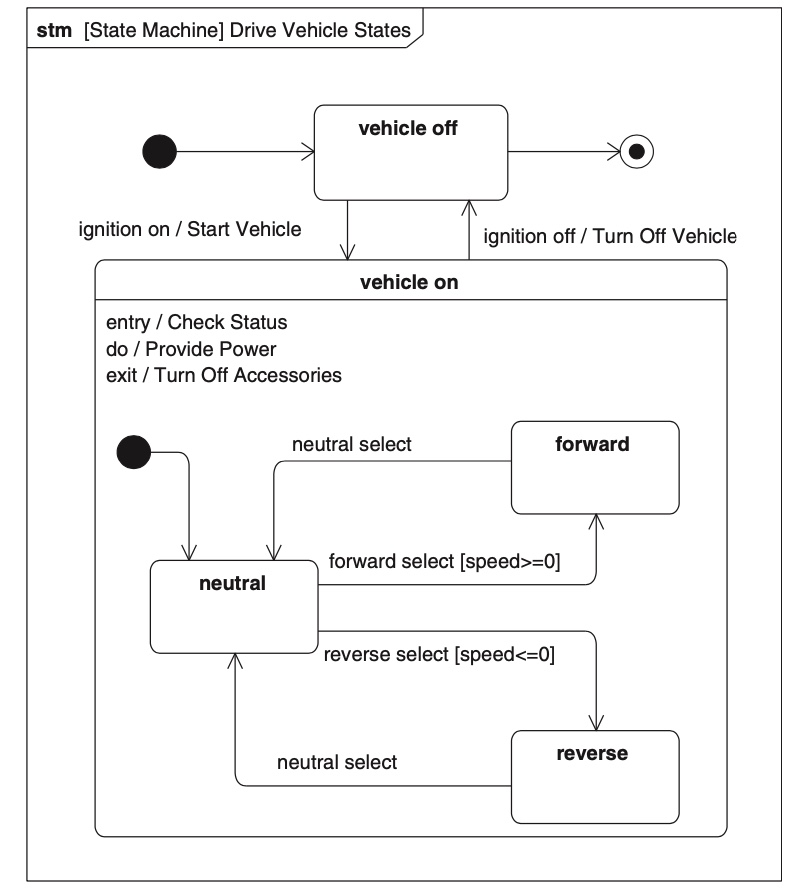
\includegraphics[width=0.75\textwidth]{figures/diagrama-maquina-estados.jpeg}
\caption{Diagrama Máquina de Estados}
\label{fig:state_machine_diagram}
\end{figure}
Na figura \ref{fig:state_machine_diagram}, pode-se observar os estados de um veículo, e também os estados quando o veículo está ligado, além dos eventos responsáveis pelas transições. 

Pode-se entender como estado a condição que determinada entidade permanece por um certo período. Já um evento é um acontecimento significativo bem determinado, no caso de máquina de estados, funcionando como gatilhos para a mudança de estado. Com essas duas definições, pode-se entender o funcionamento dos elementos do diagrama.

Como elementos importantes desse diagrama temos o círculo totalmente preenchido em preto e o círculo como outro menor dentro dele, representando, respectivamente, o estado inicial e o estado final. As setas representam as transições de estado e podem conter o evento causador dessa mudança. 

De maneira opcional, pode-se apresentar os comportamentos da entidade em determinado estado, podendo ser um comportamento realizado ao passar aquele estado, enquanto estiver nele ou ainda quando for transicionar para outro. Como pode ser observado no canto superior direito do estado do veículo ligado.

\subsubsection{Onde são utilizados com frequência}
Utilizado principalmente para descrever como um objeto muda de estado ao longo de seu tempo de vida, podendo ser uma maneira conveniente para apresentar objetos que sofrem muitas ações de diversos eventos ou ainda mostrar como certo objeto se comporta em certo caso de uso, mostrando o contexto de negócio, por exemplo. Considerando isso, permite auxiliar na modelagem de sistemas com muitas interações.

\subsection{Diagrama de Sequência}
Nesta seção será descrito o diagrama de máquina de estados, presente no SysML e também no UML. Ele é um diagrama comportamental que apresenta as interações entre sistemas ou partes do sistema.

%\subsubsection{O que é o diagrama de sequência}
%Texto

\subsubsection{Estrutura dos diagramas de sequência}
\begin{figure}[H]
\centering
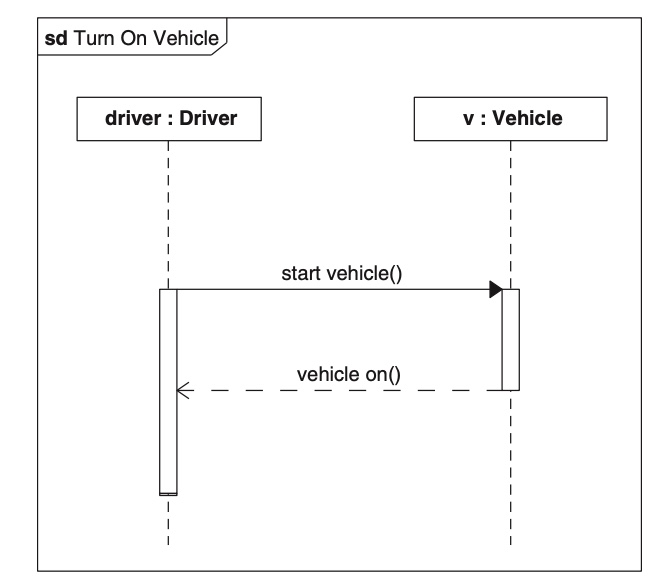
\includegraphics[width=0.75\textwidth]{figures/diagrama-sequencia.jpeg}
\caption{Diagrama de Sequência}
\label{fig:sequence_diagram}
\end{figure}
Representa as interações entre cada parte do sistema, sendo que cada parte é representada por um bloco com o nome dessa parte, cada uma possui uma linha vertical representando o tempo de vida de cada subparte durante certa interação. Na figura \ref{fig:sequence_diagram}, temos o \textit{Driver} e o \textit{Vehicle} sendo apresentados, junto com o tempo de vida de cada um. 

Pode-se indicar interações que ocorrem simultaneamente ou ainda intereações alternativas, dependendo de alguma condição apresentada. Também mostra-se nesse diagrama a troca de mensagens. 

Essa última é indicada pela utilização de setas, sendo que podem-se tratar-se de mensagens síncronas, onde espera-se uma resposta, ou mensagens assíncronas, caso contrário. Também utiliza-se uma seta diferente para representar uma resposta a uma mensagem síncrona. Na figura \ref{fig:sequence_diagram}, pode-se observar o envio da mensagem de iniciar o veículo por parte do \textit{Driver}, e a resposta do \textit{Vehicle} indicando que está ligado.

\subsubsection{Onde são utilizados com frequência}
Utilizado principalmente para representar a interação entre diferentes objetos em um determinado caso de uso, geralmente é criado nos estágios iniciais do desenvolvimento devido á sua capacidade de representar os aspectos dinâmicos do sistema, além de permitir uma revisão nos casos de uso durante a construção desse.

Além de ser usado para definir o funcionamento de determinada funcionalidade antes da implementação dessa, é útil ainda para auxiliar na compreensão de alguma já existente, caso já exista esse diagrama e ele esteja atualizado com o estado do sistema em determinado momento.

\subsection{Diagrama de Casos de Uso}
Esta seção descreve mais um dos diagramas do SysML que também existem no UML. Os diagramas de caso de uso são centrais no processo de desenvolvimento de sistemas, e normalmente são desenvolvidos no início desse processo.

\subsubsection{O que são casos de uso}

Casos de uso descrevem a funcionalidade de um sistema em termos de como ele é utilizado para atingir os objetivos de seus usuários. Os usuários de um sistema são descritos como atores, que podem representar sistemas externos ou humanos que interagem com o sistema cujo caso de uso está sendo descrito.

As relações entre o sistema, seus atores e os casos de uso é, então, descrita no diagrama de casos de uso.
Casos de uso podem também ser elaborados com descrições detalhadas de seu comportamento, fazendo uso de diagramas de Atividade, de Sequência, de Contexto ou de máquinas de estado.

Um caso de uso tipicamente cobre vários cenários, que são representados como caminhos através do caso de uso, que acontecem cada um numa circunstância diferente.

\subsubsection{Estrutura dos diagramas de casos de uso}
Os diagramas de caso de uso descrevem um conjunto de atores e de casos de uso e o relacionamento entre eles.

A figura ao fim da seção mostra um exemplo de diagrama com seus principais elementos: um sistema (Surveillance System), atores, e casos de uso, além das multiplicidades dos atores e do caso de uso. 

O pacote completo do diagrama de caso de uso pode conter diagramas que descrevem mais detalhadamente cada um dos atores envolvidos no caso de uso.

A relação entre atores e casos de uso tem características como multiplicidade. A multiplicidade do caso de uso representa com quantas instâncias do caso de uso cada ator interage por vez. A multiplicidade do lado do ator representa quantos atores podem interagir com aquele caso de uso por vez.

O exemplo abaixo mostra como os casos de uso interagem entre si utilizando as palavras-chave \textit{extend} e \textit{include}.

\begin{figure}[h]
\centering
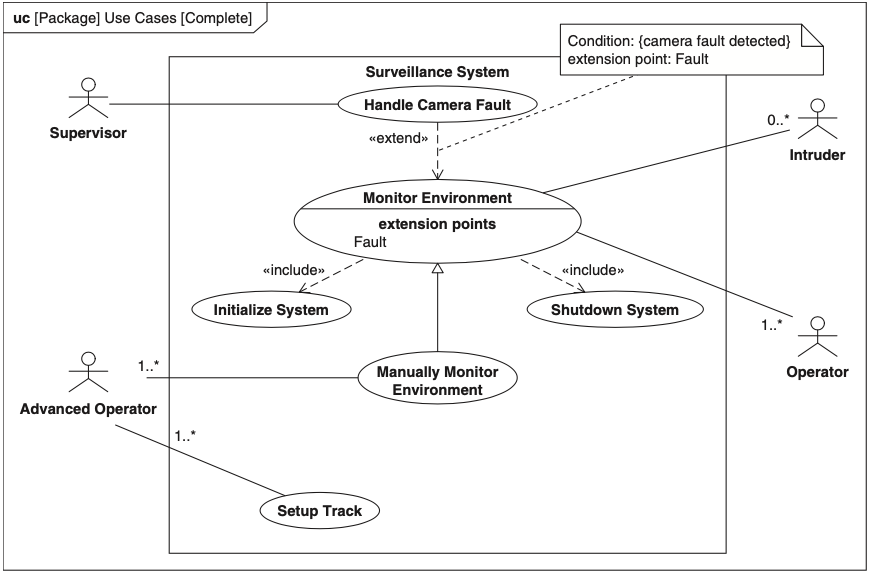
\includegraphics[width=\textwidth,height=\textheight,keepaspectratio]{figures/diagrama-caso-de-uso-3.png}
\caption{Diagrama de casos de uso}
\label{fig:use_case_diagram}
\end{figure}


\begin{itemize}
\item \textit{include}: indica que um caso de uso utiliza a funcionalidade do caso de uso ao final da seta em algum momento do seu fluxo de trabalho. 
\item \textit{extend}: indica casos de uso que realizam alguma extensão do fluxo de trabalho do caso de uso na base da seta. 
\end{itemize}

Casos de uso também podem ser descritos de maneira textual, utilizando as palavras-chave a seguir:
\begin{itemize}
\item \textbf{Pré-Condições}: Condções necessárias para o caso de uso iniciar.
\item \textbf{Pós-Condições}: Condições necessárias após o fim da execução do caso de uso.
\item \textbf{Fluxo Primário}: Fluxo de trabalho mais frequente do caso de uso
\item \textbf{Fluxos alternativos ou de exceção}: podem existir vários, e mostram o que acontece em situações menos frequentes ou em que o sistema apresenta algum erro.
\end{itemize}

\subsubsection{Onde são utilizados com frequência}

Casos de uso são a forma principal de se descrever os requisitos para um novo software sob desenvolvimento. Eles especificam o comportamento esperado do sistema.

Assim, diagramas de caso de uso são normalmente desenvolvidos nos estágios iniciais do desenvolvimento de um sistema, e, comumente, tem o propósito de especificar o contexto do sistema, capturar os requisitos do sistema, validar a arquitetura do sistema e gerar casos de teste.

Os diagramas normalmente são desenvolvidos conjuntamente por desenvolvedores de sistemas e por \textit{experts} de domínio, nas fases iniciais de levantamento de requisitos de um sistema. 

\subsection{Diagrama de Definição de Pacote}
\subsubsection{O que é diagrama de pacote}
É uma forma de organizar 

\section{Diagramas Modificados em relação ao UML}
As seções a seguir descrevem alguns dos diagramas que vieram do UML, mas foram modificados no SysML.

\section{Diagrama de Definição de Bloco}
\subsubsection{O que é diagrama de definição de blocos}

O diagrama de definições de bloco é baseado no diagrama de classes da UML com o adicional de algumas restrições e extensões definidas dentro da SysML. Sendo o diagrama mais usado dentro dessa. Sua função é modelar os aspectos estruturais, através de blocos, de um sistema, mostrando os elementos físicos, relacionamentos, fluxos e hierarquias.

\subsubsection{Estrutura dos diagramas de definição de blocos}

Com a proposta de mostrar diferentes elementos do fluxo e suas relações a figura abaixo mostra o diagrama de definição de blocos de uma ACME câmera, com os símbolos mais comuns do diagrama de blocos.


\begin{figure}[h]
\centering
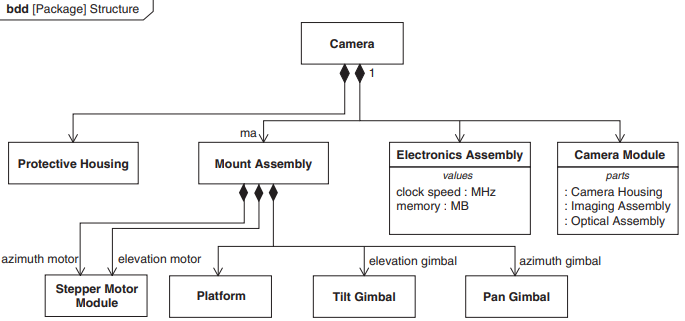
\includegraphics[width=\textwidth,height=\textheight,keepaspectratio]{figures/diagrama de blocos.PNG}
\caption{?????????????????????????}
\label{fig:block_diagram}
\end{figure}

\paragraph{}
 \textbf{Elementos físicos} 
 
 
Os elementos físicos são graficamente representados por blocos. Eles podem ser hardwares, softwares, pessoas ou qualquer outra entidade lógica ou conceitual. O nome do bloco aparece em seu topo em negrito, enquanto as outras propriedades tem seus compartimentos abaixo em letra minúscula, itálico e espaço entre as palavras. Essas propriedades podem ser de três diferentes tipos. Uma delas é propriedade de parte, que decompõem o bloco nos elementos que os constituem. Outra é a propriedade de referência, que referencia partes de outro bloco indicando em que partes o blocos conectados se relacionam. Por fim, pode-se ter também a propriedade de valor, responsável por descrever as características quantificáveis do bloco.

\paragraph{}
 \textbf{Relacionamento entre blocos} 
 
O relacionamento entre blocos indica como os blocos se relacionam, de maneira geral ele é representado com uma linha simples com elementos nas pontas, que irá indicar qual a relação exata entre eles. Existem quatro tipos diferentes de relação que podem ser representados no diagrama de blocos. 

A conexão de composição é representada graficamente por um losango preenchido conectado em um bloco maior com um traço embaixo ligando a outros blocos, é utilizado para indicar que o bloco maior possui outros elementos definindo assim uma propriedade de parte no bloco maior. Existe a possibilidade de se colocar uma seta na outra parte, neste caso faz alusão a alguma propriedade referência. 

A conexão de referência é representada graficamente por um losangolo vazio em uma ponta ligado por uma seta a outros elementos. Ela é utilizada para indicar que um bloco referencia o outro, quando existe uma referencia apenas de um lado da relação é utilizada uma seta no bloco que contém a propriedade de referência, já se ambos blocos se referenciam entre si não são utilizadas setas.

A conexão por associação pode ser utilizada tanto para definir como blocos podem estar validamente conectados quanto para detalhar essa conexão, podendo ter sua própria estrutura interna e diferentes camadas. Ela é representada por uma linha entre os dois blocos a serem conectados, ligados a uma linha tracejada partindo do meio da linha principal que leva a um terceiro bloco, responsável por detalhar a conexão. 

A conexão generalizada, indica a relação entre um bloco geral e um específico. Ela é representada graficamente por uma seta de cabeça fechada ligada ao bloco geral e uma linha simples ao bloco específico.

\paragraph{}
 \textbf{Fluxo entre os blocos} 
 
Para modelar o fluxo entre os blocos, são necessários três elementos; a porta, que representa os ponto de troca. o  fluxo de item, que define a direção que às trocas se dão e a propriedade de fluxo, irá indicar qual é a propriedade e se ela irá sair ou entrar do elemento. Assim como de conexões, existem diferentes tipos de portas. Podendo ser uma porta completa, com entrada e saída para dentro do diagrama, uma porta de proxy, onde só a entrada ou a saída estão diretamente ligadas ao diagrama ou uma porta de proxy com interface, que, onde o usuário insere a entrada no sistema. As duas primeiras são representadas por quadrados nas laterais do bloco e o último por alavancas com bolas ou semi-bolas.

    \subsubsection{Aplicação}
    
Uma aplicação para o diagrama de blocos é o uso em sistemas embarcados de tempo real. Um sistema embarcado é um sistema embutido em um hardware com um propósito de aplicação responsável por controlar e executar as funções deste hardware. Quando se trata de um sistema de tempo real, adiciona-se um grau a mais de dificuldade devido a aspectos específicos desses sistemas como mobilidade, segurança ou restrição de tempo real. Com a união de hardware e software, existe uma interação contínua com o ambiente por meio de sensores e atuadores. 

O sistema de airbag conversa com o controle de comunicação, que por sua vez extrai informações do controle de velocidade cuja a fonte são o relógio e o sensor de velocidade e do controle de peso. Estando conectado também ao controle de dashboard, responsável por comunicar o mal funcionamento do airbag. Além disso, ele recebe informações sensor e transmite para o controle de sistema do atuador que por sua vez, repassa para o atuador do airbag. Todos esses elementos e comunicações podem ser simplificados através de um digrama de definição de blocos.


\section{Diagrama de Definição de Blocos Internos}
\input{tex/Diagramas-modificados/16.2-diagrama-de-bloco-interno}

\subsection{Diagrama de Atividade}
%\subsubsection{Atividades}
Em SysML, uma atividade tem o propósito de descrever comportamento que transforma entradas em saídas, através de uma sequência de \textbf{ações}.

Ações são o bloco fundamental de descrição das atividades, mostrando como elas executam. Cada ação aceita entrada e produz saídas, que chamamos de \textbf{tokens}.

A saída de uma ação (token) se torna a entrada de outra, porque elas se conectam como peças, entrada em saída.

Fluxos de controle fornecem restrições adicionais sobre a maneira ou a ordem com que as ações que compõem uma atividade são executadas.

\subsubsection{Diagrama de Atividades}

O diagrama de atividades define as ações da atividade assim como o fluxo de entradas e saídas, e o controle entre elas. Assim, esse diagrama modela o comportamento de um caso de uso.

\begin{figure}[h]
\centering
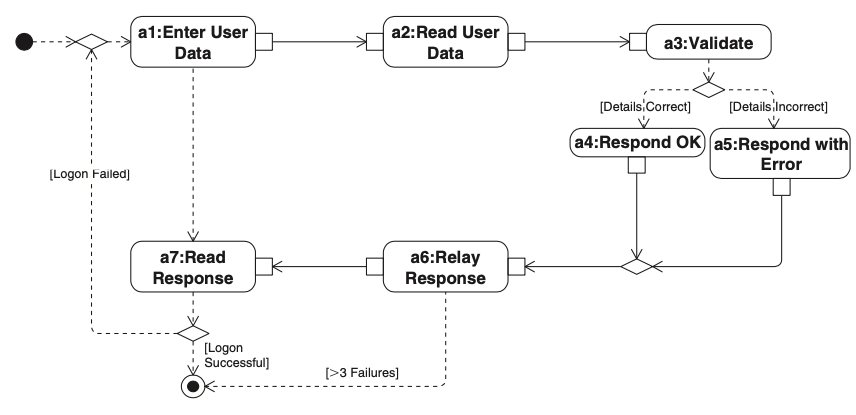
\includegraphics[width=\textwidth,height=\textheight,keepaspectratio]{figures/diagrama-atividades-1.png}
\caption{Diagrama de atividades}
\label{fig:activity_diagram}
\end{figure}
\section{Diagramas Exclusivos do SysML}
As seções a seguir descrevem alguns dos diagramas exclusivos do SysML.

\subsection{Diagrama de Definição de Parâmetros}
Diagramas de parâmetros são usados para descrever relacionamentos entre propriedades requeridas pelos sistema.

\subsubsection{Estrutura dos diagramas de parâmetros}

Os diagramas são construídos por blocos "base" e por blocos de restrição(\textit{constraints}), cada umas dessas restrições é uma equação matemática que precisa ser parametrizada.

Os blocos de restrição podem ser vinculados a constantes ou a outros blocos de restrição. Ou seja, uma restrição de um bloco pode ser o resultado dos parâmetros e restrições de outro bloco, o que permite uma visualização hierárquica das operações que precisam ser feitas.

Os Blocos são construídos por 3 partes, os parâmetros em sí:

\begin{itemize}
  \item \textbf{Nome:} Nome da restrição
  \item \textbf{Restrições:} Equações matemáticas, ou restrições vindas de outros blocos
  \item \textbf{Parâmetros:} Parâmetros a serem levados em conta nas equações 
\end{itemize}



\begin{figure}[h]
\centering
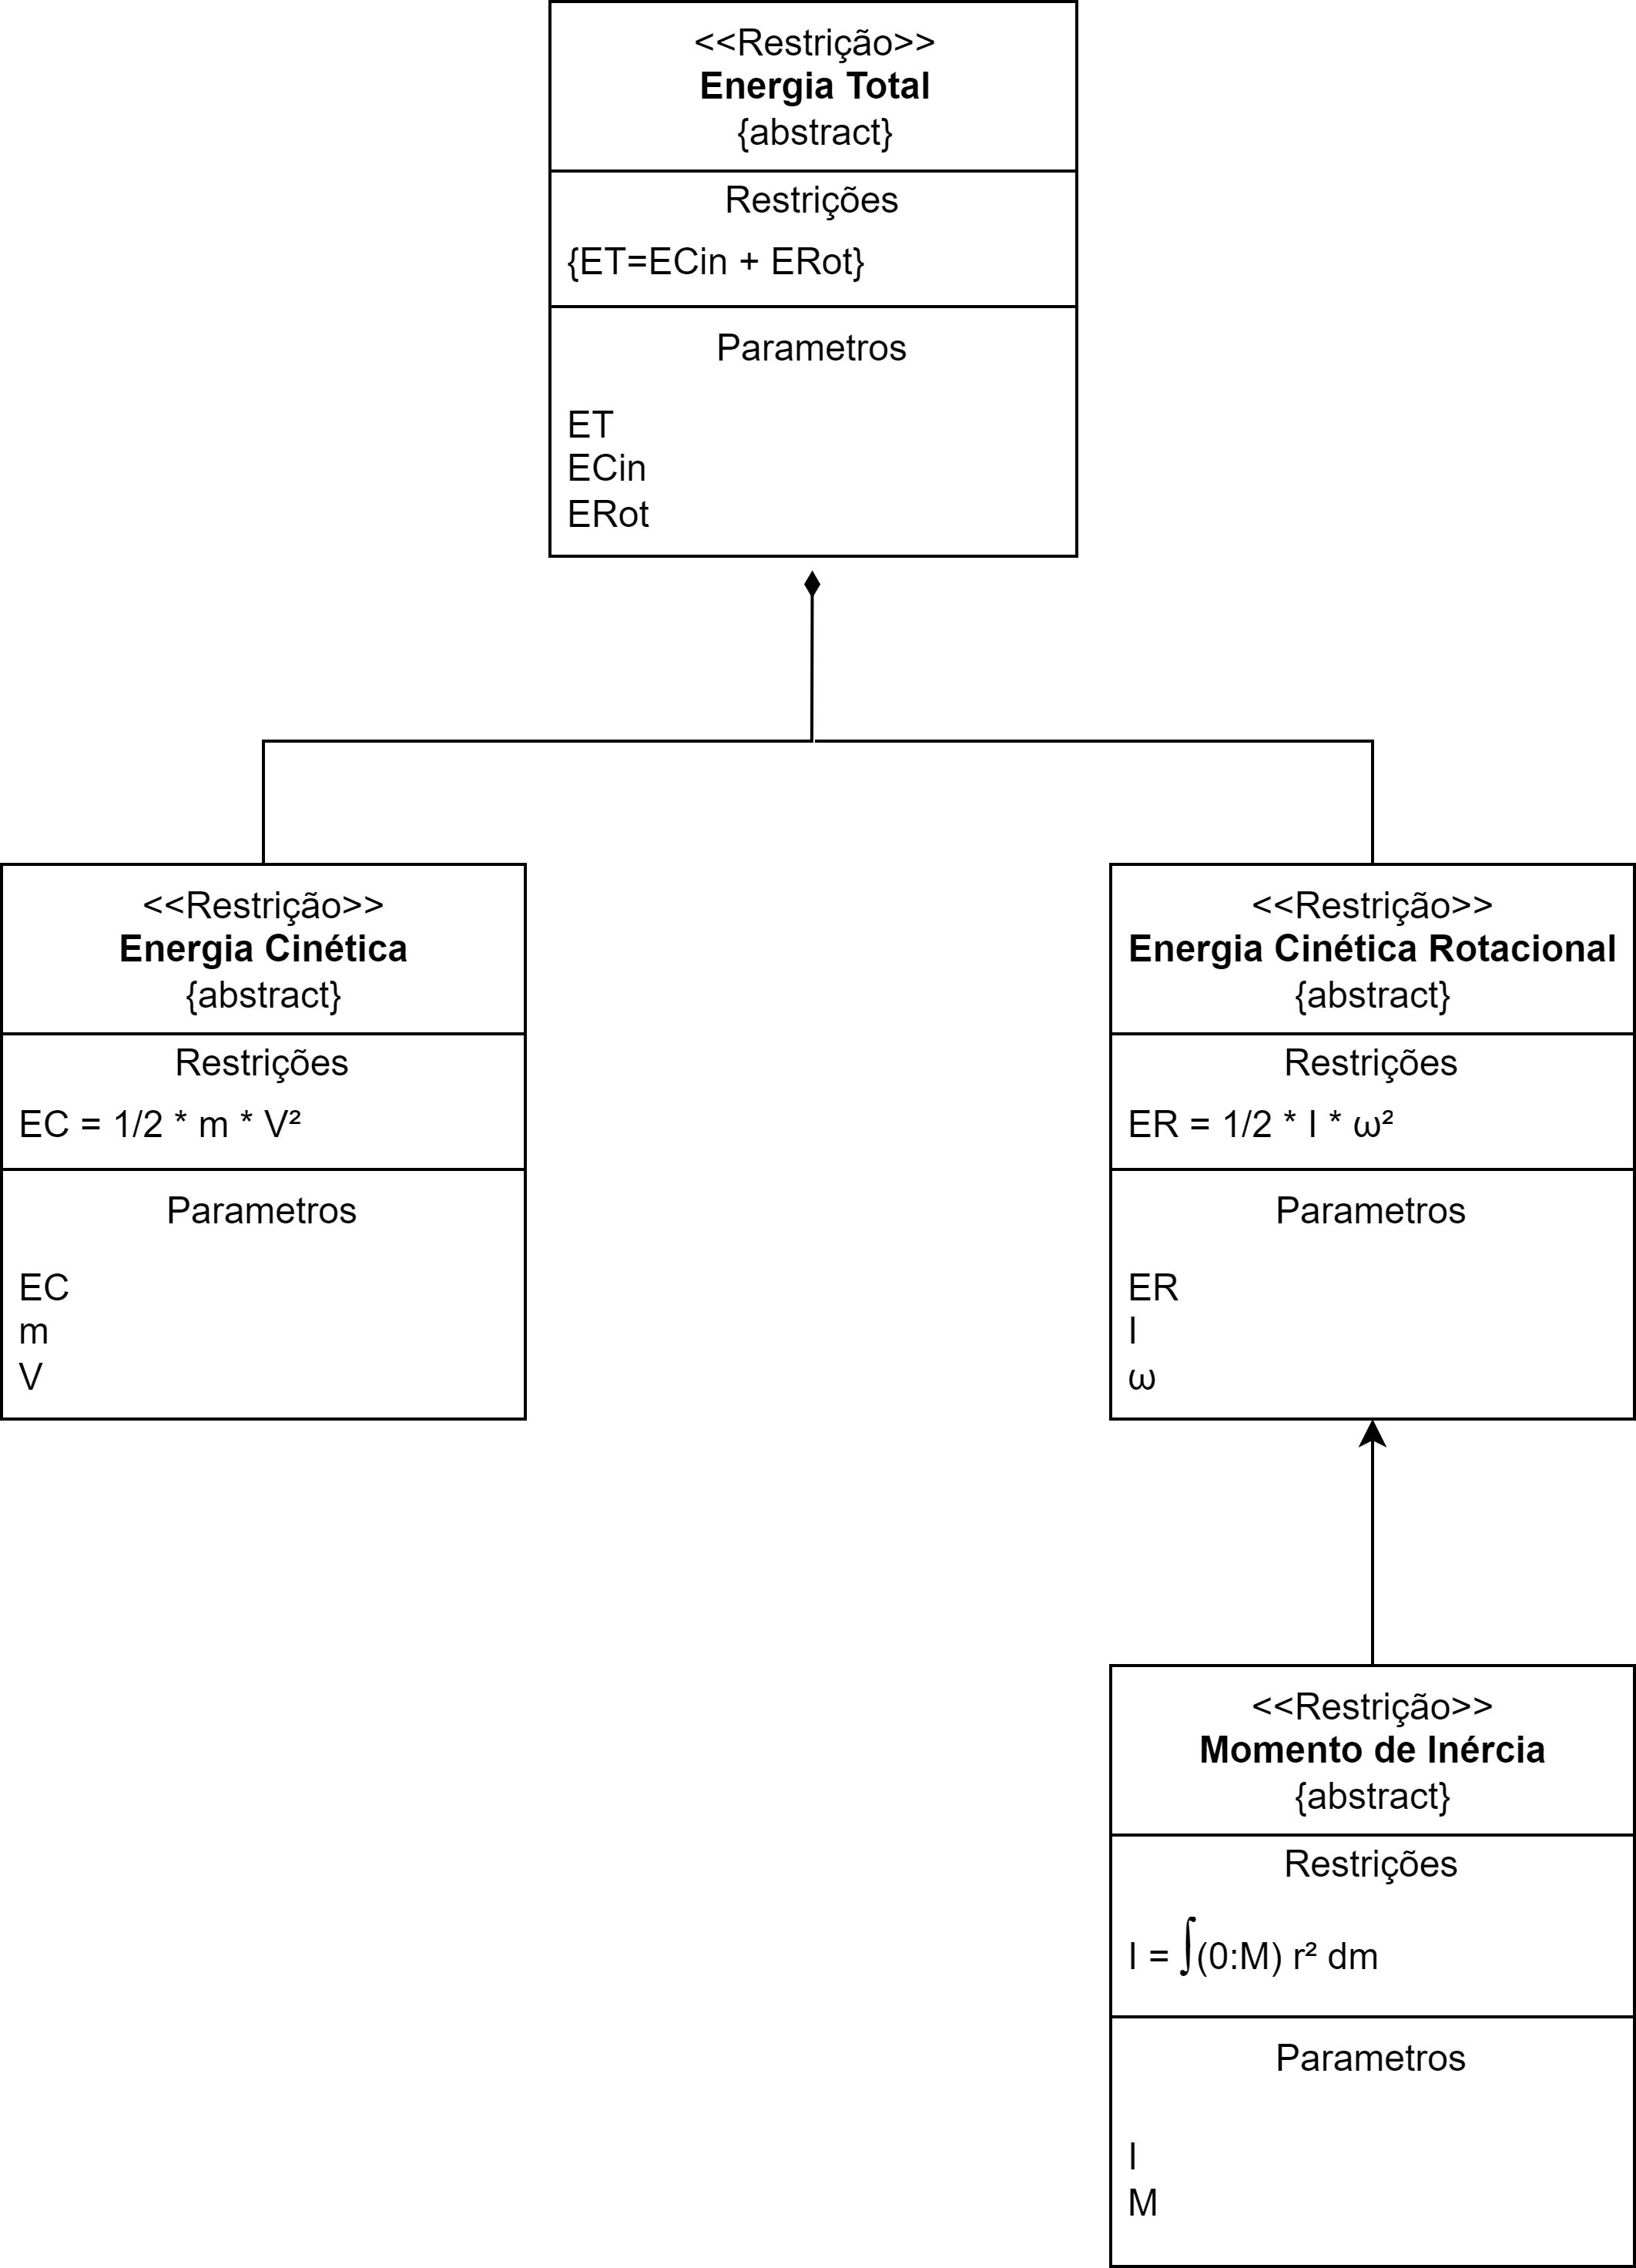
\includegraphics[width=\textwidth/2,height=\textheight,keepaspectratio]{figures/diagrama de parametros.png}
\caption{Diagrama de parâmetros}
\label{fig:parameter_diagram}
\end{figure}

\subsection{Diagrama de Definição de Requisitos}

\subsubsection{O que são requisitos}

Em suma, um requisito determina uma capacidade ou condição que deve ser satisfeita pelo sistema. Ou seja, um requisito especifica funções executadas pelo sistema ou uma qualidades que ele deve ter.

Os requisitos podem se relacionar de diversas maneiras, usando as seguintes palavras-chave:  Contém (\textit{containment}), Deriva(\textit{derive}), Satisfaz(\textit{satisfy}), Verifica(\textit{verify}), Rastreia(\textit{trace}) e Copia(\textit{copy}). De maneira geral, existe uma hierarquia entre os requisitos: alguns requisitos juntam-se para formar um requisito central mais importante.

Em SysML, há uma expansão em relação ao UML, em que requisitos podem ter relacionamentos não só entre si, mas também com elementos de design, análises e casos de testes. 


\subsubsection{Estrutura dos diagramas de requisitos}
O diagrama de requisitos representa o que é necessário para o sistema em questão funcionar conforme esperado. Seu objetivo é permitir a visualização da hierarquia e das relações entre os requisitos durante a especificação de um projeto. 

A ideia é organizar os requisitos de alto nível e baixo nível de maneira a deixar clara sua diferenciação, mas mantendo suas ligações. 

 Relações de contenção são representado por uma ligação sólida com uma cruz dentro de uma circunferência (\textit{crosshair}), as outras são relações seguem a conexão de associação detalhada em 2.2.1.

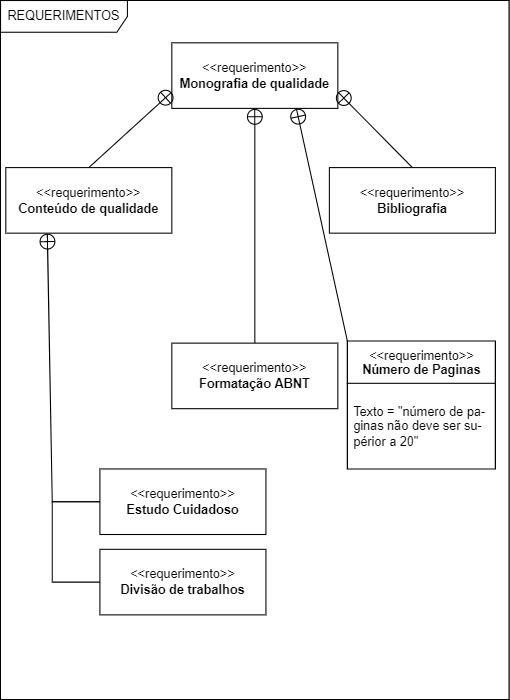
\includegraphics[width=\textwidth/2,height=\textheight,keepaspectratio]{figures/diagrama de requistos exemplo 1.png}
% \begin{figure}[h]
% \centering
% 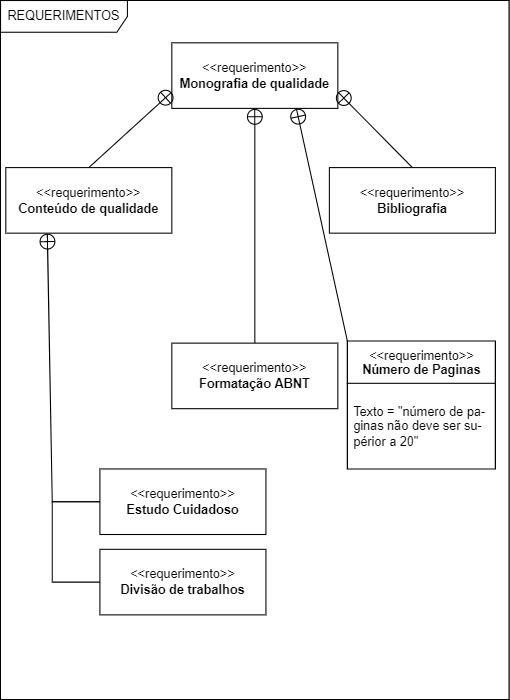
\includegraphics[width=0.75\textwidth]{figures/diagrama de requistos exemplo 1.png}
% \caption{Diagrama de Requisitos}
% \label{fig:package_diagram}
% \end{figure}


%%%%%%%%%%%%%%%%%%%%%%%%%%%%%%%%

%%%% Estilo de citação ABNT e arquivo de bibitens (mybibliography.bib)
\bibliographystyle{abnt-alf}
\bibliography{mybibliography}

\apendice
%\chapter{Título do Apêndice}
\label{Apx:A}




\chapter{Exemplo do pacote Algorithm}
\label{Apx:B}


\begin{algorithm}[!h]
\caption{Estimador ML otimizado.}\label{Alg:MAXVER}
\begin{algorithmic}[1]
\STATE Inicializar o contador: $j\leftarrow 1$;%
\STATE Fixar o limiar de variação das estimativas: $e_{\mathrm{out}}\leftarrow 10^{-4}$;%
\STATE Fixar o número máximo de iterações: $N\leftarrow 1000$;%
\STATE Computar o ponto inicial: $\hat \gamma(0)$;%
\STATE Determinar o limiar inicial: $e_1 \leftarrow1000$;%
\STATE Estabelecer o valor inicial de $\alpha$: $\hat \alpha(0) \leftarrow -10^{-6}$;%
\WHILE{ $e_j \geq e_{\mathrm{out}}$ e $ j\leq M$}
    \STATE Solucionar $\hat \alpha_j\leftarrow {\arg \max}_{\alpha}\;{l_1(\alpha; \gamma_{j-1},\mathbf{z},n)}$;%
    \STATE Solucionar $\hat \gamma_j\leftarrow {\arg \max}_{\gamma}\;{l_2(\gamma; \alpha_j,\mathbf{z},n)}$;%
    \STATE $j\leftarrow j+1$
    \STATE Computar o critério de convergência: $e_j$;%
\ENDWHILE
\end{algorithmic}
\end{algorithm}


\end{document}